% The code is quite messy !!!

\documentclass[tikz,border=10pt]{standalone}

\begin{document}

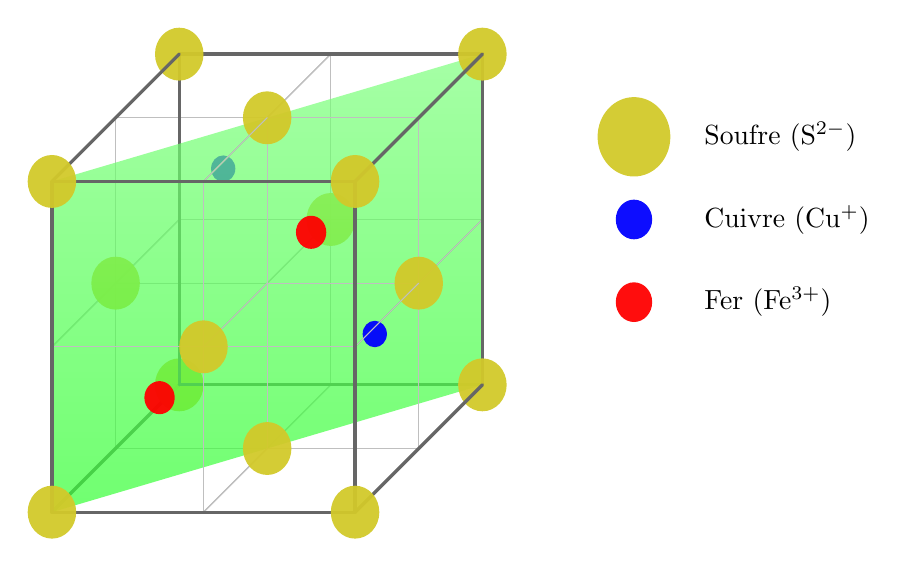
\begin{tikzpicture}[scale=3.5, x={(1.1,0)}, y={(0,1.2)}, z={(0, 0, 1.2)}, line join=round, line cap=round]

    % site tetra arriere
    \fill[blue, opacity=0.95] (0.25,0.75,0.25) circle (0.04); % Tetrahedral sites

    % Edges of the small cubes (a/2)
    \foreach \x in {0, 0.5, 1} {
        \foreach \y in {0, 0.5, 1} {
            \foreach \z in {0, 0.5, 1} {
                % Draw edges of each small cube
                \draw[lightgray, thin] (\x,\y,0) -- (\x,\y,1); % vertical edges
                \draw[lightgray, thin] (\x,0,\z) -- (\x,1,\z); % edges parallel to y-axis
                \draw[lightgray, thin] (0,\y,\z) -- (1,\y,\z); % edges parallel to x-axis
            }
        }
    }

    \draw[black!60, very thick] (0,0,0) -- (0,0,1);  % cube edge


    \fill[yellow!80!black, opacity=0.95] (0,0,0) circle (0.08);
    \fill[yellow!80!black, opacity=0.95] (0.5,0.5,0) circle (0.08);
    \fill[yellow!80!black, opacity=0.95] (0,0.5,0.5) circle (0.08);

    \draw[black!60, very thick] (0,0,0) -- (1,0,0); % face arriere
    \draw[black!60, very thick] (0,0,0) -- (0,1,0); % face arriere

    % plan de coupe
    \shade[top color=green!50, bottom color=green!80, opacity=0.7] (0,0,1) -- (0,1,1) -- (1,1,0) -- (1,0,0) -- cycle;
    %  \fill[green, opacity=0.5] (0,0,1) -- (0,1,1) -- (1,1,0) -- (1,0,0) -- cycle;

    \fill[blue, opacity=0.95] (0.75,0.25,0.25) circle (0.04); % Tetrahedral sites

    \foreach \x/\y/\z in {0.5/0.5/0.5, 0.5/0/0.5}{
        % Draw edges of each small cube
        \draw[lightgray, thin] (\x,\y,\z) -- (\x+0.5,\y,\z) -- (\x+0.5,\y+0.5,\z) -- (\x,\y+0.5,\z) -- cycle; % face arriere
        \draw[lightgray, thin] (\x,\y,\z+0.5) -- (\x+0.5,\y,\z+0.5) -- (\x+0.5,\y+0.5,\z+0.5) -- (\x,\y+0.5,\z+0.5) -- cycle; % face avant
        \draw[lightgray, thin] (\x,\y,\z) -- (\x,\y,\z+0.5);
    }


    \draw[lightgray, thin] (0,0.5,1) -- (0.5,0.5,1);
    \draw[lightgray, thin] (1,0.5,0) -- (1,0.5,0.5);

    % Cube edges (main cube)
    \draw[black!60, very thick] (1,0,0) -- (1,1,0) -- (0,1,0); % face arriere
    
    % Vertices of the main cube (face arriere)
     \foreach \x/\y/\z in {1/0/0, 1/1/0, 0/1/0, 0.5/0/0.5} {
        \fill[yellow!80!black, opacity=0.95] (\x,\y,\z) circle (0.08);
    }

    
    \draw[black!60, very thick] (1,0,0) -- (1,0,1);  % cube edge
    \draw[black!60, very thick] (1,1,0) -- (1,1,1);  % cube edge
    \draw[black!60, very thick] (0,1,0) -- (0,1,1);  % cube edge

    % site tetra avant
    \foreach \x/\y/\z in {0.25/0.25/0.75, 0.75/0.75/0.75} {
        \fill[red, opacity=0.95] (\x,\y,\z) circle (0.05);
    }


    % cube top face verteses and right face
    \fill[yellow!80!black, opacity=0.95] (0.5,1,0.5) circle (0.08);
    \fill[yellow!80!black, opacity=0.95] (1,0.5,0.5) circle (0.08);

    \draw[lightgray, thin] (0.5,1,0.5) -- (0.5,1,1);
    \draw[lightgray, thin] (1,0.5,0.5) -- (1,0.5,1);

    % Cube edges face avant
    \draw[black!60, very thick] (0,0,1) -- (1,0,1) -- (1,1,1) -- (0,1,1) -- cycle; 

    % Vertices of the main cube (face avant)
    \foreach \x/\y/\z in {0/0/1, 1/0/1, 1/1/1, 0/1/1, 0.5/0.5/1} {
        \fill[yellow!80!black, opacity=0.95] (\x,\y,\z) circle (0.08);
    }

     % Légende des atomes
     \begin{scope}[shift={(1.5,0)}] % Décalage à droite pour placer la légende

        % Soufre (S²⁻)
        \fill[yellow!80!black, opacity=0.95] (0,0.75) circle (0.12);
        \node[right] at (0.2,0.75) {Soufre (S$^{2-}$)};

        % Cuivre (Cu⁺)
        \fill[blue, opacity=0.95] (0,0.5) circle (0.06);
        \node[right] at (0.2,0.5) {Cuivre (Cu$^+$)};

        % Fer (Fe³⁺)
        \fill[red, opacity=0.95] (0,0.25) circle (0.06);
        \node[right] at (0.2,0.25) {Fer (Fe$^{3+}$)};
        
    \end{scope}

\end{tikzpicture}

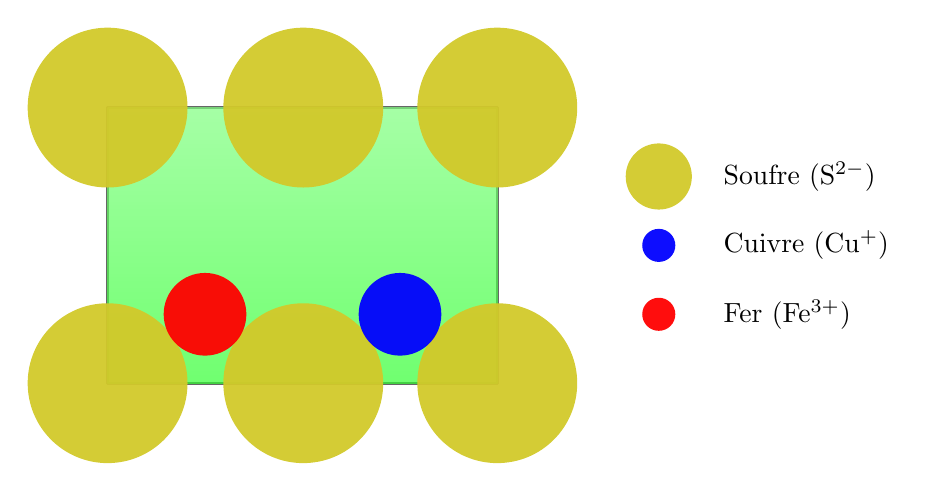
\begin{tikzpicture}[scale=3.5, line join=round, line cap=round]
    % rectangle edges (main cube)
    \draw[black!60, very thick] (0,0) rectangle ({sqrt(2)}, 1);
    \shade[top color=green!50, bottom color=green!80, opacity=0.7] (0,0) rectangle ({sqrt(2)}, 1);

     \foreach \x/\y in {0/0, 1.414/0, 1.414/1, 0/1, 0.71/1, 0.71/0} {
        \fill[yellow!80!black, opacity=0.95] (\x,\y) circle (0.29);  % atomes S
    }

    \fill[red, opacity=0.95] (0.3535,0.25) circle (0.15);  % atome cuivre
    \fill[blue, opacity=0.95] (1.061,0.25) circle (0.15);  %  atome fer

    % Légende des atomes
    \begin{scope}[shift={(2,0)}] % Décalage à droite pour placer la légende

        % Soufre (S²⁻)
        \fill[yellow!80!black, opacity=0.95] (0,0.75) circle (0.12);
        \node[right] at (0.2,0.75) {Soufre (S$^{2-}$)};

        % Cuivre (Cu⁺)
        \fill[blue, opacity=0.95] (0,0.5) circle (0.06);
        \node[right] at (0.2,0.5) {Cuivre (Cu$^+$)};

        % Fer (Fe³⁺)
        \fill[red, opacity=0.95] (0,0.25) circle (0.06);
        \node[right] at (0.2,0.25) {Fer (Fe$^{3+}$)};
        
    \end{scope}

\end{tikzpicture}

\end{document}
